%!TEX TS-program = xelatex
%!TEX encoding = UTF-8 Unicode

%%
%% 使用 njuthesis 文档类生成南京大学本科生毕业论文的示例文档
%%
%% 作者:张楚珩,zhangchuheng123 (at) live (dot) com
%% 个人主页: http://sealzhang.tk
%%

%% 
%% 感谢Hu Haixing提供的南京大学硕博学位论文模板
%% 项目主页:http://haixing-hu.github.io/nju-thesis/
%%

\documentclass{njuthesis}

%%%%%%%%%%%%%%%%%%%%%%%%%%%%%%%%%%%%%%%%%%%%%%%%%%%%%%%%%%%%%%%%%%%%%%%%%%%%%%%
% 设置论文的中文封面

% 论文标题
\title{高举中国特色社会主义伟大旗帜}

% 论文作者姓名
\author{张海豹}
% 论文作者学号
\studentid{121120000}
% 导师姓名职称
\supervisor{费曼~~教授}
% 论文作者的学科与专业方向
\major{物理学院光电科学系}
% 论文作者的研究方向
\researchfield{量子通讯与量子计算}
% 论文的定稿日期,需设置年、月、日。此属性可选,默认值为最后一次编译时的日期,精确到日。
% \date{2013年5月1日}

%%%%%%%%%%%%%%%%%%%%%%%%%%%%%%%%%%%%%%%%%%%%%%%%%%%%%%%%%%%%%%%%%%%%%%%%%%%%%%%
% 设置论文的英文封面

% 论文的英文标题
\englishtitle{A Research on Network Infrastructures for Data Centers}
% 论文作者姓名的拼音
\englishauthor{WEI Xiao-Bao}
% 导师姓名职称的英文
\englishsupervisor{Professor CHEN Jin-Nan}
% 论文作者所在院系的英文名称
\englishdepartment{Department of Physics}
% 论文作者所在学校或机构的英文名称。此属性可选,默认值为``Nanjing University''。
\englishinstitute{Nanjing University}
% 论文完成日期的英文形式,默认最后一次编译的时间
% \englishdate{May 1, 2013}

\begin{document}

% 制作中文封面
\maketitle
% 制作英文封面
\makeenglishtitle

% 论文的中文摘要
\begin{abstract}
中国共产党第十六次全国代表大会,是我们党在新世纪召开的第一次代表大会,也是我们党在开始实施社会主义现代化建设第三步战略部署的新形势下召开的一次十分重要的代表大会。 

大会的主题是:高举邓小平理论伟大旗帜,全面贯彻”三个代表”重要思想,继往开来,与时俱进,全面建设小康社会,加快推进社会主义现代化,为开创中国特色社会主义事业新局面而奋斗。 

当人类社会跨入二十一世纪的时候,我国进入全面建设小康社会、加快推进社会主义现代化的新的发展阶段。国际局势正在发生深刻变化。世界多极化和经济全球化的趋势在曲折中发展,科技进步日新月异,综合国力竞争日趋激烈。形势逼人,不进则退。我们党必须坚定地站在时代潮流的前头,团结和带领全国各族人民,实现推进现代化建设、完成祖国统一、维护世界和平与促进共同发展这三大历史任务,在中国特色社会主义道路上实现中华民族的伟大复兴。这是历史和时代赋予我们党的庄严使命。 

同时应该注意到,空白页是故意留白,以便章节开头能够出现在偶数页。
% 中文关键词。关键词之间用中文全角分号隔开,末尾无标点符号。
\keywords{江泽民;中国共产党;第十七届全国代表大会}
\end{abstract}

%%%%%%%%%%%%%%%%%%%%%%%%%%%%%%%%%%%%%%%%%%%%%%%%%%%%%%%%%%%%%%%%%%%%%%%%%%%%%%%
% 论文的英文摘要
\begin{englishabstract}
This is the test for the English abstract.
% 英文关键词。关键词之间用英文半角逗号隔开,末尾无符号。
\englishkeywords{Small World, Network Model, Data Center}
\end{englishabstract}

%%%%%%%%%%%%%%%%%%%%%%%%%%%%%%%%%%%%%%%%%%%%%%%%%%%%%%%%%%%%%%%%%%%%%%%%%%%%%%%
% 论文的前言,应放在目录之前,中英文摘要之后
%
\begin{preface}

十五大以来的五年,是我们高举邓小平理论伟大旗帜不断开拓创新的五年,是我们经受住各种困难和风险的考验、继续沿着中国特色社会主义道路胜利前进的五年。 

十五大确立邓小平理论为党的指导思想,提出党在社会主义初级阶段的基本纲领,明确了我国跨世纪发展的奋斗目标和任务。为贯彻十五大精神,中央先后召开七次全会,分别就农业和农村工作、国有企业改革和发展、制定”十五”计划、加强和改进党的作风建设等重大问题,作出决定和部署。五年来,我们走过了很不平凡的历程,在改革发展稳定、内政外交国防、治党治国治军各方面都取得了巨大成就。 

国民经济持续快速健康发展。实施扩大内需的方针,适时采取积极的财政政策和稳健的货币政策,克服亚洲金融危机和世界经济波动对我国的不利影响,保持了经济较快增长。经济结构战略性调整取得成效,农业的基础地位继续加强,传统产业得到提升,高新技术产业和现代服务业加速发展。建设了一大批水利、交通、通信、能源和环保等基础设施工程。西部大开发取得重要进展。经济效益进一步提高,财政收入不断增长。“九五”计划胜利完成,“十五”计划开局良好。 

改革开放取得丰硕成果。社会主义市场经济体制初步建立。公有制经济进一步壮大,国有企业改革稳步推进。个体、私营等非公有制经济较快发展。市场体系建设全面展开,宏观调控体系不断完善,政府职能转变步伐加快。财税、金融、流通、住房和政府机构等改革继续深化。开放型经济迅速发展,商品和服务贸易、资本流动规模显著扩大。国家外汇储备大幅度增加。我国加入世贸组织,对外开放进入新阶段。 

社会主义民主政治和精神文明建设成效显著。民主法制建设继续推进,政治体制改革迈出新步伐。爱国统一战线发展壮大,民族、宗教和侨务工作取得新进展。社会治安综合治理取得新成效。科技、教育、文化、卫生、体育和计划生育等事业全面进步。宣传舆论工作和思想道德建设不断加强,群众精神文化生活日益丰富。 

国防和军队建设迈出新步伐。人民解放军的革命化现代化正规化建设继续加强,国防实力和军队防卫作战能力进一步提高。军队、武警和民兵在保卫和建设祖国中发挥了重要作用。 

人民生活总体上达到小康水平。城乡居民收入稳步增长。城乡市场繁荣,商品供应充裕,居民生活质量提高,衣食住用行都有较大改善。社会保障体系建设成效明显。“八七”扶贫攻坚计划基本完成。 

祖国统一大业取得新进展。我国政府恢复对澳门行使主权。坚持贯彻“一国两制”方针,严格执行香港特别行政区基本法和澳门特别行政区基本法,香港和澳门社会经济稳定。海峡两岸人员往来和经济文化交流不断加强。反对”台独”等各种分裂图谋的斗争深入开展。 

对外工作开创新局面。根据国际形势的发展变化,坚持正确的对外方针和政策,广泛开展双边和多边外交,积极参与国际交流和合作,我国的国际地位进一步提高。 

\vspace{1cm}
\begin{flushright}
江泽民\\
2002年11月8日于人民大会堂
\end{flushright}

\end{preface}

%%%%%%%%%%%%%%%%%%%%%%%%%%%%%%%%%%%%%%%%%%%%%%%%%%%%%%%%%%%%%%%%%%%%%%%%%%%%%%%
% 生成论文目录
\tableofcontents

%%%%%%%%%%%%%%%%%%%%%%%%%%%%%%%%%%%%%%%%%%%%%%%%%%%%%%%%%%%%%%%%%%%%%%%%%%%%%%%
% 生成插图清单。如无需插图清单则可注释掉下述语句。
\listoffigures

%%%%%%%%%%%%%%%%%%%%%%%%%%%%%%%%%%%%%%%%%%%%%%%%%%%%%%%%%%%%%%%%%%%%%%%%%%%%%%%
% 生成附表清单。如无需附表清单则可注释掉下述语句。
\listoftables

%%%%%%%%%%%%%%%%%%%%%%%%%%%%%%%%%%%%%%%%%%%%%%%%%%%%%%%%%%%%%%%%%%%%%%%%%%%%%%%
% 开始正文部分
\mainmatter

%%%%%%%%%%%%%%%%%%%%%%%%%%%%%%%%%%%%%%%%%%%%%%%%%%%%%%%%%%%%%%%%%%%%%%%%%%%%%%%
% 学位论文的正文应以《绪论》作为第一章
\chapter{绪论}\label{chapter_introduction}
\section{研究背景}

对外工作开创新局面。根据国际形势的发展变化,坚持正确的对外方针和政策,广泛开展双边和多边外交,积极参与国际交流和合作,我国的国际地位进一步提高。 

党的建设全面加强。全党对邓小平理论的学习不断深入。我们提出并深刻阐述了”三个代表”重要思想。”三讲”集中教育和”三个代表”学习教育活动卓有成效。党的思想、组织、作风建设全面推进,思想政治工作得到加强。干部制度改革迈出新步伐。廉政建设和反腐败斗争深入开展,取得新的明显成效。


\section{研究目的与意义}
\subsection{现有解决方法}
\begin{table}[htbp]
  \centering
  \begin{tabular}{cccp{38mm}}
    \toprule
    \textbf{文档域类型} & \textbf{Java类型} & \textbf{宽度(字节)} & \textbf{说明} \\
    \midrule
    BIG\_INTEGER & java.math.BigInteger & 和具体值有关 & 任意精度的长整数 \\
    BIG\_DECIMAL & java.math.BigDecimal & 和具体值有关 & 任意精度的十进制实数 \\
    \bottomrule
  \end{tabular}
  \caption{测试表格}\label{table:test1}
\end{table}
\subsection{现有问题与不足}

测试一下引用\cite{newman2006structure},连续引用
\cite{newman2001random,aiello2000random,bollobas2001random},另一个连续引用
\cite{newman2001random,bollobas2001random,barabasi1999emergence}。测试一下带页码
的引用\cite[124--128]{erdHos1961strength}。

贯彻”三个代表”重要思想,必须把发展作为党执政兴国的第一要务,不断开创现代化建设的新局面。马克思主义执政党必须高度重视解放和发展生产力。离开发展,坚持党的先进性、发挥社会主义制度的优越性和实现民富国强都无从谈起。党的先进性是具体的、历史的,必须放到推动当代中国先进生产力和先进文化的发展中去考察,放到维护和实现最广大人民根本利益的奋斗中去考察,归根到底要看党在推动历史前进中的作用。 

我们党在中国这样一个经济文化落后的发展中大国领导人民进行现代化建设,能不能解决好发展问题,直接关系人心向背、事业兴衰。党要承担起推动中国社会进步的历史责任,必须始终紧紧抓住发展这个执政兴国的第一要务,把坚持党的先进性和发挥社会主义制度的优越性,落实到发展先进生产力、发展先进文化、实现最广大人民的根本利益上来,推动社会全面进步,促进人的全面发展。紧紧把握住这一点,就从根本上把握了人民的愿望,把握了社会主义现代化建设的本质,就能使”三个代表”重要思想不断落实,使党的执政地位不断巩固,使强国富民的要求不断得到实现。 

发展必须坚持以经济建设为中心,立足中国现实,顺应时代潮流,不断开拓促进先进生产力和先进文化发展的新途径。发展必须坚持和深化改革。一切妨碍发展的思想观念都要坚决冲破,一切束缚发展的做法和规定都要坚决改变,一切影响发展的体制弊端都要坚决革除。发展必须相信和依靠人民,人民是推动历史前进的动力。要集中全国人民的智慧和力量,聚精会神搞建设,一心一意谋发展。 

\chapter{结论}

\begin{figure}[htbp]
   \centering
   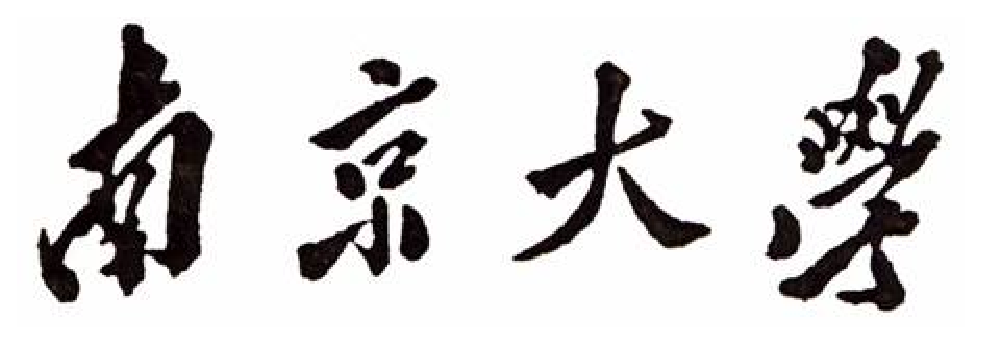
\includegraphics[width=0.7\textwidth]{njuname.eps} % requires the graphicx package
   \caption{测试图片}
   \label{fig:example}
\end{figure}

贯彻”三个代表”重要思想,必须把发展作为党执政兴国的第一要务,不断开创现代化建设的新局面。马克思主义执政党必须高度重视解放和发展生产力。离开发展,坚持党的先进性、发挥社会主义制度的优越性和实现民富国强都无从谈起。党的先进性是具体的、历史的,必须放到推动当代中国先进生产力和先进文化的发展中去考察,放到维护和实现最广大人民根本利益的奋斗中去考察,归根到底要看党在推动历史前进中的作用。 

我们党在中国这样一个经济文化落后的发展中大国领导人民进行现代化建设,能不能解决好发展问题,直接关系人心向背、事业兴衰。党要承担起推动中国社会进步的历史责任,必须始终紧紧抓住发展这个执政兴国的第一要务,把坚持党的先进性和发挥社会主义制度的优越性,落实到发展先进生产力、发展先进文化、实现最广大人民的根本利益上来,推动社会全面进步,促进人的全面发展。紧紧把握住这一点,就从根本上把握了人民的愿望,把握了社会主义现代化建设的本质,就能使”三个代表”重要思想不断落实,使党的执政地位不断巩固,使强国富民的要求不断得到实现。 

发展必须坚持以经济建设为中心,立足中国现实,顺应时代潮流,不断开拓促进先进生产力和先进文化发展的新途径。发展必须坚持和深化改革。一切妨碍发展的思想观念都要坚决冲破,一切束缚发展的做法和规定都要坚决改变,一切影响发展的体制弊端都要坚决革除。发展必须相信和依靠人民,人民是推动历史前进的动力。要集中全国人民的智慧和力量,聚精会神搞建设,一心一意谋发展。 

贯彻”三个代表”重要思想,必须把发展作为党执政兴国的第一要务,不断开创现代化建设的新局面。马克思主义执政党必须高度重视解放和发展生产力。离开发展,坚持党的先进性、发挥社会主义制度的优越性和实现民富国强都无从谈起。党的先进性是具体的、历史的,必须放到推动当代中国先进生产力和先进文化的发展中去考察,放到维护和实现最广大人民根本利益的奋斗中去考察,归根到底要看党在推动历史前进中的作用。 

我们党在中国这样一个经济文化落后的发展中大国领导人民进行现代化建设,能不能解决好发展问题,直接关系人心向背、事业兴衰。党要承担起推动中国社会进步的历史责任,必须始终紧紧抓住发展这个执政兴国的第一要务,把坚持党的先进性和发挥社会主义制度的优越性,落实到发展先进生产力、发展先进文化、实现最广大人民的根本利益上来,推动社会全面进步,促进人的全面发展。紧紧把握住这一点,就从根本上把握了人民的愿望,把握了社会主义现代化建设的本质,就能使”三个代表”重要思想不断落实,使党的执政地位不断巩固,使强国富民的要求不断得到实现。 

发展必须坚持以经济建设为中心,立足中国现实,顺应时代潮流,不断开拓促进先进生产力和先进文化发展的新途径。发展必须坚持和深化改革。一切妨碍发展的思想观念都要坚决冲破,一切束缚发展的做法和规定都要坚决改变,一切影响发展的体制弊端都要坚决革除。发展必须相信和依靠人民,人民是推动历史前进的动力。要集中全国人民的智慧和力量,聚精会神搞建设,一心一意谋发展。 

贯彻”三个代表”重要思想,必须把发展作为党执政兴国的第一要务,不断开创现代化建设的新局面。马克思主义执政党必须高度重视解放和发展生产力。离开发展,坚持党的先进性、发挥社会主义制度的优越性和实现民富国强都无从谈起。党的先进性是具体的、历史的,必须放到推动当代中国先进生产力和先进文化的发展中去考察,放到维护和实现最广大人民根本利益的奋斗中去考察,归根到底要看党在推动历史前进中的作用。 

我们党在中国这样一个经济文化落后的发展中大国领导人民进行现代化建设,能不能解决好发展问题,直接关系人心向背、事业兴衰。党要承担起推动中国社会进步的历史责任,必须始终紧紧抓住发展这个执政兴国的第一要务,把坚持党的先进性和发挥社会主义制度的优越性,落实到发展先进生产力、发展先进文化、实现最广大人民的根本利益上来,推动社会全面进步,促进人的全面发展。紧紧把握住这一点,就从根本上把握了人民的愿望,把握了社会主义现代化建设的本质,就能使”三个代表”重要思想不断落实,使党的执政地位不断巩固,使强国富民的要求不断得到实现。 

发展必须坚持以经济建设为中心,立足中国现实,顺应时代潮流,不断开拓促进先进生产力和先进文化发展的新途径。发展必须坚持和深化改革。一切妨碍发展的思想观念都要坚决冲破,一切束缚发展的做法和规定都要坚决改变,一切影响发展的体制弊端都要坚决革除。发展必须相信和依靠人民,人民是推动历史前进的动力。要集中全国人民的智慧和力量,聚精会神搞建设,一心一意谋发展。 

\bibliography{sample}

%%%%%%%%%%%%%%%%%%%%%%%%%%%%%%%%%%%%%%%%%%%%%%%%%%%%%%%%%%%%%%%%%%%%%%%%%%%%%%%
% 致谢,应放在结论之后
\begin{acknowledgement}
以改革的精神推进党的建设,还必须按改革的规律办事,以科学的态度对待改革、推进改革。党的建设是一件政治性、政策性很强的系统工程。研究和解决党的建设中的各种重大问题,既需要全党同志的积极努力,又要坚持集中和统一的领导。不能自行其是,一哄而起。党的建设的各种措施和办法,都要有计划、有组织、有步骤地推行。有的,还要经过试点,取得经验,制定规章,再逐步推广。要注意防止出现思想上的片面性,不能刮风。如果不采取科学的态度,就会出现这样那样的问题,反而影响党的建设的顺利进行。
\end{acknowledgement}

%%%%%%%%%%%%%%%%%%%%%%%%%%%%%%%%%%%%%%%%%%%%%%%%%%%%%%%%%%%%%%%%%%%%%%%%%%%%%%%
\end{document}
